%%%%%%%%%%%%%%%%%%%%%%%%%%%%%%%%%%%%%%%%%
% Beamer Presentation
% LaTeX Template
% Version 1.0 (10/11/12)
%
% This template has been downloaded from:
% http://www.LaTeXTemplates.com
%
% License:
% CC BY-NC-SA 3.0 (http://creativecommons.org/licenses/by-nc-sa/3.0/)
%
%%%%%%%%%%%%%%%%%%%%%%%%%%%%%%%%%%%%%%%%%

%----------------------------------------------------------------------------------------
%	PACKAGES AND THEMES
%----------------------------------------------------------------------------------------

\documentclass{beamer}

\mode<presentation> {

% The Beamer class comes with a number of default slide themes
% which change the colors and layouts of slides. Below this is a list
% of all the themes, uncomment each in turn to see what they look like.

%\usetheme{default}
%\usetheme{AnnArbor}
%\usetheme{Antibes}
%\usetheme{Bergen}
%\usetheme{Berkeley}
%\usetheme{Berlin}
%\usetheme{Boadilla}
%\usetheme{CambridgeUS}
%\usetheme{Copenhagen}
%\usetheme{Darmstadt}
%\usetheme{Dresden}
%\usetheme{Frankfurt}
%\usetheme{Goettingen}
%\usetheme{Hannover}
%\usetheme{Ilmenau}
%\usetheme{JuanLesPins}
%\usetheme{Luebeck}
\usetheme{Madrid}
%\usetheme{Malmoe}
%\usetheme{Marburg}
%\usetheme{Montpellier}
%\usetheme{PaloAlto}
%\usetheme{Pittsburgh}
%\usetheme{Rochester}
%\usetheme{Singapore}
%\usetheme{Szeged}
%\usetheme{Warsaw}

% As well as themes, the Beamer class has a number of color themes
% for any slide theme. Uncomment each of these in turn to see how it
% changes the colors of your current slide theme.

%\usecolortheme{albatross}
%\usecolortheme{beaver}
%\usecolortheme{beetle}
%\usecolortheme{crane}
%\usecolortheme{dolphin}
%\usecolortheme{dove}
%\usecolortheme{fly}
%\usecolortheme{lily}
%\usecolortheme{orchid}
%\usecolortheme{rose}
%\usecolortheme{seagull}
%\usecolortheme{seahorse}
%\usecolortheme{whale}
%\usecolortheme{wolverine}

%\setbeamertemplate{footline} % To remove the footer line in all slides uncomment this line
%\setbeamertemplate{footline}[page number] % To replace the footer line in all slides with a simple slide count uncomment this line

%\setbeamertemplate{navigation symbols}{} % To remove the navigation symbols from the bottom of all slides uncomment this line
}

\usepackage{graphicx} % Allows including images
\usepackage{booktabs} % Allows the use of \toprule, \midrule and \bottomrule in tables

%----------------------------------------------------------------------------------------
%	TITLE PAGE
%----------------------------------------------------------------------------------------

\title[Open Aircraft Design]{Open Source Aircraft Design} % The short title appears at the bottom of every slide, the full title is only on the title page

\author{Niel Agenbag} % Your name
\institute[Unaffiliated] % Your institution as it will appear on the bottom of every slide, may be shorthand to save space
{
University of California \\ % Your institution for the title page
\medskip
\textit{john@smith.com} % Your email address
}
\date{\today} % Date, can be changed to a custom date

\begin{document}

\begin{frame}
\titlepage % Print the title page as the first slide
\end{frame}

\begin{frame}
\frametitle{Overview} % Table of contents slide, comment this block out to remove it
\tableofcontents % Throughout your presentation, if you choose to use \section{} and \subsection{} commands, these will automatically be printed on this slide as an overview of your presentation
\end{frame}

%----------------------------------------------------------------------------------------
%	PRESENTATION SLIDES
%----------------------------------------------------------------------------------------

%------------------------------------------------
\section{First Section} % Sections can be created in order to organize your presentation into discrete blocks, all sections and subsections are automatically printed in the table of contents as an overview of the talk
%------------------------------------------------

\subsection{Subsection Example} % A subsection can be created just before a set of slides with a common theme to further break down your presentation into chunks

\begin{frame}
\frametitle{Paragraphs of Text}
Aircraft design requires specialist knowledge and skills.  Furthermore large capital investment is required, often with little guarantee of return on investment and often at low margins.  Things have changed though, with remotely piloted vehicles that can reduce risk, open source software, first person view, collaboration tools (GIT). \\~\\

Doing what hobbyists have been doing for years, exchanging components and expertise, but over the internet that facilitates the scaling of the design and analysis process.


Make it possible to commit CAD files via Python scripting

Enable trade of skills and equipment in an open way.

This removes the hysteresis (marketing department, sales, HR) associated with companies with large overheads.  Projects can easily spend money but bringing money in is difficult.
Pure trade (classical horse trading) immediately negates the losses associated with the existing system.

\end{frame}

%------------------------------------------------

\begin{frame}
\frametitle{Bullet Points}

Many tools are required for designing, analysing and building an aircraft.  The following typical tools are required.  A libre, open source example of each is presented next to the type of software.

\begin{itemize}
\item Computer aided design (CAD) tools - FreeCAD
\item Finite element analysis - Calculix (bundled with FreeCAD) or Nastran95, Code Aster
\item Computational fluid dynamics (CFD) - OpenFOAM (also integrated with FreeCAD)
\item Rigid body dynamic simulation - Project Chrono
\item General matrix computation, large data processing for flight testing - Python
\item Version control - Git
\item Product lifecycle management - Combination of Git and a browser based framework such as Django (not yet developed, but envisaged)
\end{itemize}
\end{frame}

%------------------------------------------------

%------------------------------------------------

\begin{frame}
\frametitle{Philosophy begin FOSS}

Free Open Source Software (FOSS) has some of its roots with the Free Software Foundation that started life at MIT and was responsible for one of the first and certainly one of the longest lasting text environments called emacs.

FOSS does in part democratize software and makes it transparent for everyone to use and edit with very few restrictions.

The implication of libre software is that it enables innovation by lowering the barriers to entry and standardizing methods all across the globe.

This might not seem very important at face value, but it has great consequences that have not been fully realized yet.

The fact that libre software is available at no cost or lag (the time it takes to release software) has the following consequences:

\begin{itemize}
\item Skilled engineers that previously had little or no access to high end engineering software are now free to innovate
\item Libre software allows proper scaling to be possible, meaning that the number of engineers that can work on a problem is now only limited by the number of engineers you can find and not by license restrictions
\item The scaling of the engineering profession will have an exponential effect on innovation
\item It enables engineers to use complexity to their advantage since these packages enables more and more complex analyses
\item Libre software provide a way of levelling the playing field with respect to engineering input costs, although it put a premium on skills, since engineers using it usually need more knowledge than the average user of paid software, since there is less technical support.
\item Software development can happen in parallel on a 24/7 basis with contributors from around the world.  This is facilitated by tools like Git.
\end{itemize}

\end{frame}

%------------------------------------------------

%------------------------------------------------

\begin{frame}
\frametitle{Philosophy begin FOSS}

The scaling effect of libre software is not as immediately apparent as it should be.  Let us explain by means of an analogy.
Let us examine a common system of metrology such as the metric system or the imperial system.
Up to 1920's many countries had different definitions of an inch.
Gauge blocks were invented in 1896 by Swedish machinist Carl Edvard Johansson.
To a large degree these gauge blocks standardized the industrial inch and also could be used for the metric system.

The gauge blocks made it possible for different machine shops, companies and indeed countries to have standard references of measurement.

This might not seem immediately apparent, but this enables a global scalable manufacturing system.  Lego blocks made in Chech republic fits onto blocks made in the U.S. and not only that, they fit onto blocks made thirty years ago.

You can manufacture more, quicker than ever before at higher quality.

\end{frame}

%------------------------------------------------


\begin{frame}
\frametitle{Philosophy begin FOSS}

What is the relevance of gauge blocks to libre software?
The answer is that libre software is the gauge blocks of the software industry.
All engineers in the world have the opportunity to use standard and benchmarked methods that have taken thousands of hours to develop.

They can share their ideas globally and scale on a level that has never been seen before.
All this without sacrificing flexibility, since standard methods can be forked and custom developed (while possibly later standardizing itself).  All the while the body of tools can grow.

You can analyze and engineer more products, quicker than ever before at higher quality.

\end{frame}



\begin{frame}
\frametitle{Philosophy begin FOSS}

Gauge blocks standardized measurement and brought metrology out into the open.  This meant that specialized knowledge was not limited to companies or in a previous time, guilds.

Similarly libre software brings advanced analysis to any engineer willing to try and use the software.  It is now not limited to companies (in essence macro guilds) with large software budgets.

Standardization increased the gross product of manufacturing immensely over the last century leading to great prosperity for the entities that embraced it.

Libre software has the possiblility of providing just such a platform for innovation to scale exponentially.  Also with the accompanying properity and increase in gross product.
This will be aided by collaborative platforms such as Github that facilitates the large scale sharing of information, methods and contact between engineers.

Thus facilitating the free movement of ideas, intellectual (and consequently monetary) capital and contact between persons.

\end{frame}



%------------------------------------------------

\begin{frame}
\frametitle{Mechanical/Aeronautical Engineering as coding discipline}

The lines are blurring between engineering and software coding.

Engineering a product has become a software excercise.  For example, in FreeCAD a whole component can be constructed using python commands.  The versions of the CAD document can be controlled by Git, since the script file is a text file.
The analysis can fully be performed in a text python file.  Or the finite element analysis can be scripted using a text file.
The results from the FEA run produces large amounts of data, that is once again manipulated by using software tools.

Engineering has become inseparable from software development.

As such it is important to adopt software methodologies in order to manage engineering projects, such as agile project management.  And to adopt the fail early, fail often, fail safe approach.

This has been shown to most degrees to be successful at SpaceX and Tesla.


\end{frame}

%------------------------------------------------


\begin{frame}
\frametitle{Blocks of Highlighted Text}
\begin{block}{Block 1}
Lorem ipsum dolor sit amet, consectetur adipiscing elit. Integer lectus nisl, ultricies in feugiat rutrum, porttitor sit amet augue. Aliquam ut tortor mauris. Sed volutpat ante purus, quis accumsan dolor.
\end{block}

\begin{block}{Block 2}
Pellentesque sed tellus purus. Class aptent taciti sociosqu ad litora torquent per conubia nostra, per inceptos himenaeos. Vestibulum quis magna at risus dictum tempor eu vitae velit.
\end{block}

\begin{block}{Block 3}
Suspendisse tincidunt sagittis gravida. Curabitur condimentum, enim sed venenatis rutrum, ipsum neque consectetur orci, sed blandit justo nisi ac lacus.
\end{block}
\end{frame}

%------------------------------------------------

\begin{frame}
\frametitle{Multiple Columns}
\begin{columns}[c] % The "c" option specifies centered vertical alignment while the "t" option is used for top vertical alignment

\column{.45\textwidth} % Left column and width
\textbf{Heading}
\begin{enumerate}
\item Statement
\item Explanation
\item Example
\end{enumerate}

\column{.5\textwidth} % Right column and width
Lorem ipsum dolor sit amet, consectetur adipiscing elit. Integer lectus nisl, ultricies in feugiat rutrum, porttitor sit amet augue. Aliquam ut tortor mauris. Sed volutpat ante purus, quis accumsan dolor.

\end{columns}
\end{frame}

%------------------------------------------------
\section{Second Section}
%------------------------------------------------

\begin{frame}
\frametitle{Table}
\begin{table}
\begin{tabular}{l l l}
\toprule
\textbf{Treatments} & \textbf{Response 1} & \textbf{Response 2}\\
\midrule
Treatment 1 & 0.0003262 & 0.562 \\
Treatment 2 & 0.0015681 & 0.910 \\
Treatment 3 & 0.0009271 & 0.296 \\
\bottomrule
\end{tabular}
\caption{Table caption}
\end{table}
\end{frame}

%------------------------------------------------

\begin{frame}
\frametitle{Theorem}
\begin{theorem}[Mass--energy equivalence]
$E = mc^2$
\end{theorem}
\end{frame}

%------------------------------------------------

\begin{frame}[fragile] % Need to use the fragile option when verbatim is used in the slide
\frametitle{Verbatim}
\begin{example}[Theorem Slide Code]
\begin{verbatim}
\begin{frame}
\frametitle{Theorem}
\begin{theorem}[Mass--energy equivalence]
$E = mc^2$
\end{theorem}
\end{frame}\end{verbatim}
\end{example}
\end{frame}

%------------------------------------------------

\begin{frame}
\frametitle{Figure}
Metric gauge blocks from Wikipedia.
\begin{figure}
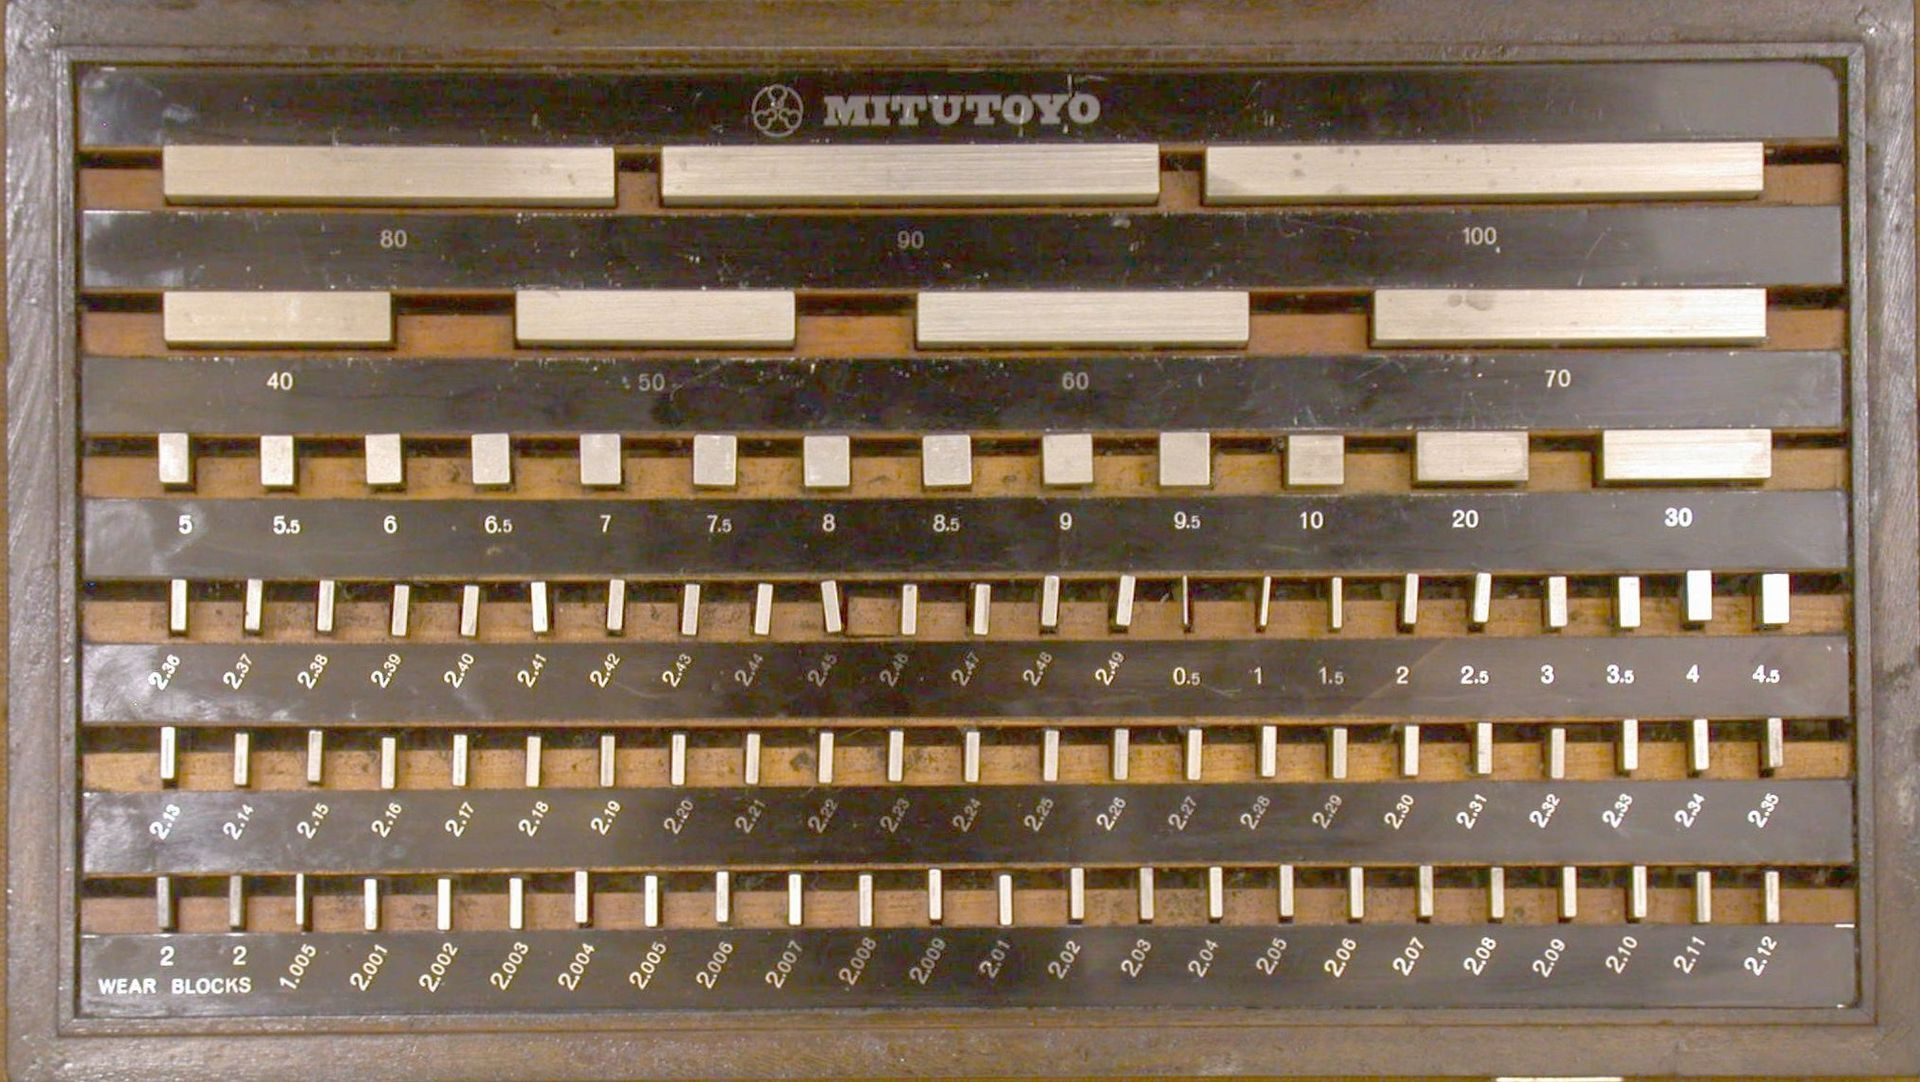
\includegraphics[width=0.8\linewidth]{GaugeBlockMetricSet.jpg}
\end{figure}
\end{frame}

%------------------------------------------------

\begin{frame}[fragile] % Need to use the fragile option when verbatim is used in the slide
\frametitle{Citation}
An example of the \verb|\cite| command to cite within the presentation:\\~

This statement requires citation \cite{p1}.
\end{frame}

%------------------------------------------------

\begin{frame}
\frametitle{References}
\footnotesize{
\begin{thebibliography}{99} % Beamer does not support BibTeX so references must be inserted manually as below
\bibitem[Smith, 2012]{p1} John Smith (2012)
\newblock Title of the publication
\newblock \emph{Journal Name} 12(3), 45 -- 678.
\end{thebibliography}
}
\end{frame}

%------------------------------------------------

\begin{frame}
\Huge{\centerline{The End}}
\end{frame}

%----------------------------------------------------------------------------------------

\end{document} 